\chapter{Przedstawienie omawianych technologii}
Ten rozdział poświęcony jest omówieniu używanych technologii i pojęć w pozostałych rozdziałach.
\section{Aplikacja monolityczna}

\begin{figure}[h!]
  \centering
    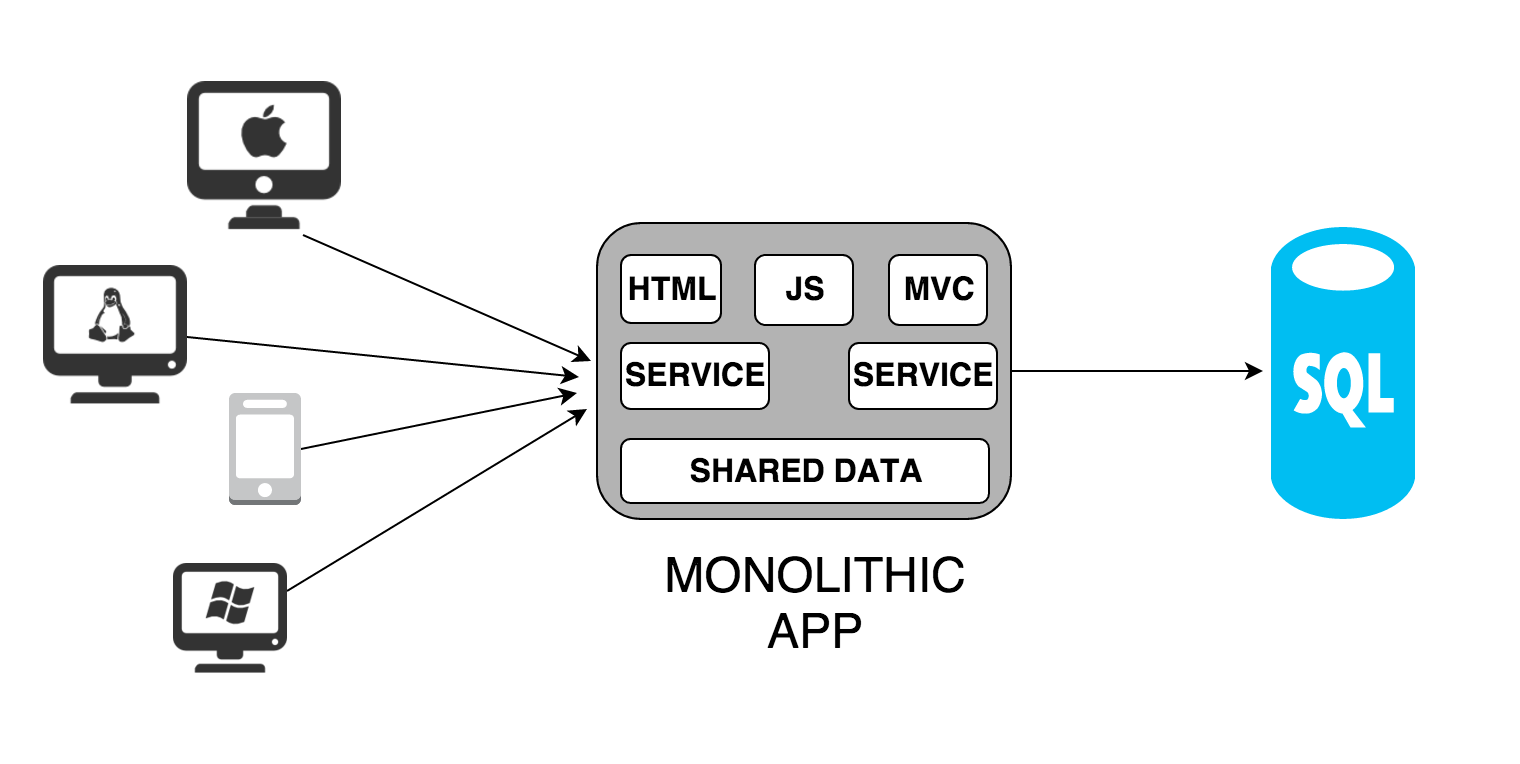
\includegraphics[width=0.8\textwidth]{images/monolithic-arch.png}
  \caption{Architektura monolityczna. Źródło: \cite{MonolitVsMicro} }
\end{figure}

W inżynierii oprogramowania monolityczna aplikacja\index{aplikacja monolityczna} to taka, która została zaprojektowana bez modułowości.\cite{Monolit2}

Aplikacja monolityczna\index{aplikacja monolityczna} to sposób budowania systemów informatycznych, w którym wszystkie komponenty działają w ramach jednej aplikacji. Dawniej popularny ze względu na brak realnych alternatyw — aplikacje działały na komputerach typu mainframe, a chmura obliczeniowa była wymysłem futurystów.

Takie podejście do tworzenia aplikacji ma zalety m.in:
\begin{itemize}
    \item Nie dotyczą jej problemy związane z komunikacją sieciową.
    \item Wymiana danych pomiędzy modułami może odbywać się w pamięci.
    \item Nie ma problemów ze spójnością danych.
\end{itemize}

Minusem jest bardzo ograniczona możliwość skalowania — tego rodzaju aplikacje często bardzo trudno przenieść na wiele równolegle działających komputerów.\cite{Monolit1}

\section{Aplikacja mikroserwisowa}
\begin{figure}[h!]
  \centering
    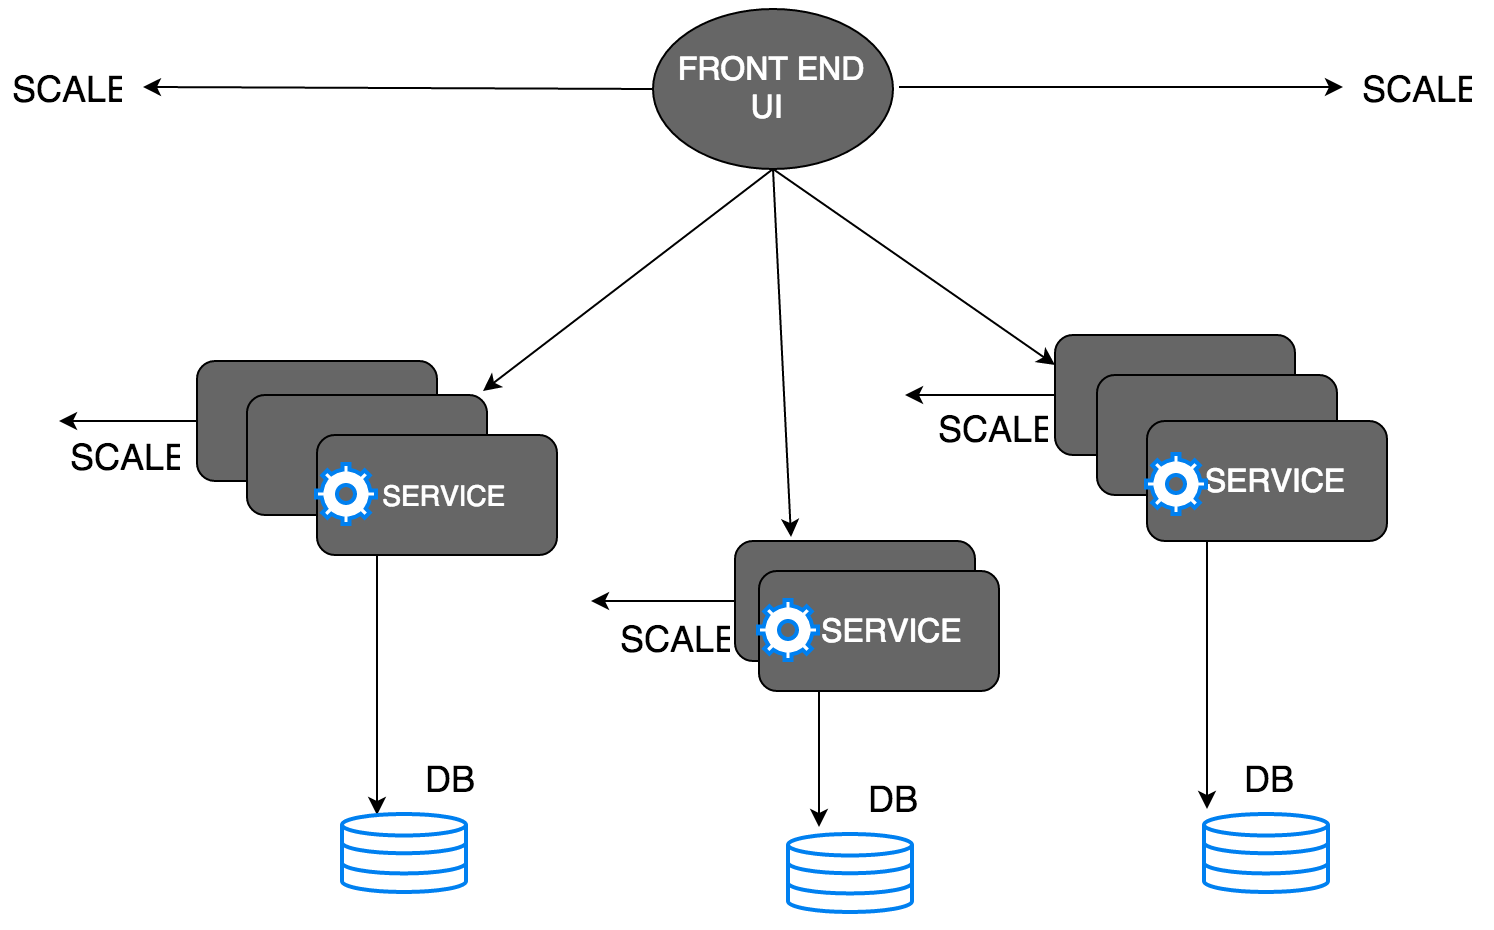
\includegraphics[width=0.8\textwidth]{images/microservice-arch.png}
  \caption{Architektura Mikroserwisowa. Źródło: \cite{MonolitVsMicro} }
\end{figure}
Mikroserwisy to styl programowania, w którym zespolone aplikacje składają się z wielu niezależnych serwisów. Serwisy są rozdzielone i skupione na spełnianiu niewielkich zadań – mogą być one oddzielnie rozwijane, testowane, budowane i lokowane. Koncepcja mikrousług wywodzi się z SOA – architektury zorientowanej na usługi, która swoje triumfy święciła wiele lat temu. Teraz powraca w ulepszonej postaci właśnie jako mikrousługi.\cite{Micro1}

Każdy mikroserwis jest stosunkowo mały, co daje wiele zalet, ale również i wad.

Do zalet \cite{Micro2} należą:
\begin{itemize}
    \item Kod jest łatwiejszy do zrozumienia przez programistę.
    \item Stanowi mniejsze obiążenie dla zintegrowanego środowiska programistycznego.
    \item Pozwala na szybszy start kontenera aplikacji.
    \item Każdy mikroserwis można dostarczać niezależnie od innych serwisów, z różnym cyklem wydawniczym włącznie.
    \item Każdy mikroserwis można wytwarzać w innym zespole w innej lokalizacji nawet przy użyciu innych narzędzi, technologii i języków.
    \item Każdy mikroserwis działa jako odrębna aplikacja, proces, czy instancja maszyny wirtualnej, wiec problemy wewnętrzne w samym kontenerze nie wpływają na działanie innych serwisów.
\end{itemize}

Do wad \cite{Micro2} należą:
\begin{itemize}
    \item Komplikuje się proces wytwarzania systemu, system staje się zbiorem małych systemów, które trzeba zgrać i zsynchronizować.
    \item Testowanie, choć jednostkowo prostsze w układzie testowania całego złożonego systemu, jest wyraźnie trudniejsze ze znaczną rozbudową testów integracyjnych.
    \item Transakcje to potencjalny problem tejże architektury, w sytuacji kiedy transakcje rozpinają się ponad mikroserwisami.
\end{itemize}

,,Zalety i wady mikroserwisów są oczywiste i trudno z nimi dyskutować, jednak warto jak zawsze zdefiniować kontekst. Jaki mamy projekt, jakie wymagania, które z wad aplikują się do naszego przypadku, które z korzyści na nas spłyną, czy w naszym przypadku to się opłaci.''\cite{Micro2}

\section{Anemic Model}
Anemiczny model\index{Anemic Model} aplikacji to antywzorzec projektowy, często wystepujący przy tworzeniu aplikacji monolitycznych\index{aplikacja monolityczna} opartych o scentralizowaną bazę danych, wykorzystujące operacje CRUD\index{CRUD} czyli dodawaniu, odczytywaniu, aktualizacji i usuwaniu informacji.

Aplikacje oparte na modelu anemicznym\index{Anemic Model} to takie, które opierają się na operacjach bazodanowych i nie są niczym innym jak jedynie oprawą graficzną dla struktury bazy danych. Użytkownik owego system opartego na tym modelu, władający wiedzą z zakresu baz danych, potrafiłby bezpośrednio na poziomie połączenia z bazą danych zmieniać stan danych aplikacji adekwatnie do potrzeb logiki biznesowej, co byłoby w wielu przypadkach równoznaczne z użyciem zaprojektowanego systemu opartego na tej bazie.

Jest to jeden z antyzworców projektowych.
,,W tym przypadku model dziedziny składa się z klas z atrybutami bez metod, nie jest więc obiektowy. Logika biznesowa przeniesiona jest do innych klas, które transformują klasy dziedziny zmieniając ich stan (...) Antywzorzec ten jest przedmiotem wielu dyskusji – znaczna część metodyk tworzenia oprogramowania w Javie (w tym EJB) operuje na takim modelu. Duża część projektantów przenosi też swoje przyzwyczajenia z modelowania baz danych modelując system w ten sposób.''\cite{Antywzorzec-projektowy}

\section{Event Sourcing}
Event Sourcing\index{Event Sourcing} opiera cały system na wydarzeniach (Event), które zapisywane są trwale do bazy danych (Sourcing). 

W innych modelach, opierających się na relacyjnych lub nierelacyjnych bazach danych i operacjach CRUD\index{CRUD}, skupiamy się jedynie na stanie aktualnym aplikacji. Jakakolwiek aktualizacja czy usunięcie danych zmienia dane w sposób trwały i tracimy informację o wcześniejszej wersji danej sprzed aktualizacji czy usunięcia.

Taka informacja może być bardzo przydatna z paru powodów:
\begin{itemize}
    \item Specyfikacja domenowa często wymaga zachowania pełnej wersji wydarzeń w systemie. Jednym z przykładów byłyby banki, gdzie każda transakcja musi być zapisana. Innym przykładem są sklepy internetowe, które chcą lepiej zrozumieć zachowanie klienta na stronie. Klient może dodać produkt do koszyka, potem go z niego usunąć i dokonać zakupu innych produktów. Aplikacja w wersji nieopartej na wydarzeniach nie zapisze stanu pośredniego, a jedynie stan końcowy z produktami kupionymi przez użytkownika. Event Sourcing\index{Event Sourcing} pomaga na zapisanie każdej najmniejszej czynności, opisanej w wymaganiach biznesowych.
    \item Posiadanie całej historii danych w aplikacji może pozwolić nam na  odtworzenie wszystkich operacji od początku lub cofnięcie się w czasie do danego momentu w razie potrzeby. Ta możliwość jest również charakterystyczna dla systemów opratych o Blockchain, który ma wiele wspólnego z Event Sourcing'iem\index{Event Sourcing} pod tym wzgledem.
    \item Możemy szybko rozpoznać i zabezpieczyć system przed sytuacjami niebezpiecznymi i atakami osób trzecich na dane aplikacji.
\end{itemize}

,,Zamiast koncentrować się na bieżącym stanie, koncentrujesz się na zmianach, które zaszły w czasie. Jest to praktyka modelowania systemu jako sekwencji zdarzeń.''\cite{EventSourcing1}


\begin{figure}[h!]
  \centering
    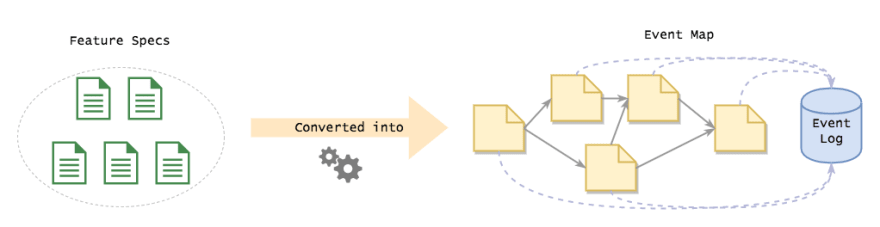
\includegraphics[width=1.0\textwidth]{images/eventsourcing.png}
  \caption{Zapis wydarzeń w systemie. Źródło: \cite{EventSourcing1} }
\end{figure}

Każda akcja w aplikacji (ang. Feature Specs) zapisywana jest jako wydarzenie (Event) w tzw. Event Log, czyli bazie danych wydarzeń, która traktowana jest jako źródło prawdy całego systemu.

Bardzo ważną cechą Event Sourcing'u\index{Event Sourcing} jest sposób na późniejsze przygotowanie i prezentację danych użytkownikowi systemu.

Jeśli każdy stan aplikacji pochodzi od zdarzeń, w jaki sposób możemy pobierać dane, które muszą być prezentowane użytkownikowi? Czy za każdym razem musimy pobierać wszystkie zdarzenia i budować zestaw danych?

\begin{figure}[h!]
  \centering
    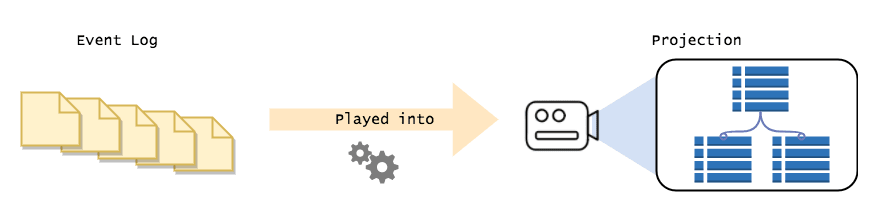
\includegraphics[width=1.0\textwidth]{images/eventsourcing2.png}
  \caption{Odczyt danych z wydarzeń poprzez projekcję. Źródło: \cite{EventSourcing1} }
\end{figure}

,,Wyniki budowane są w tle, przechowując resultaty pośrednie w bazie danych. W ten sposób użytkownicy mogą wyszukiwać dane, a otrzymają je w dokładnie takim kształcie, jakiego potrzebują, z minimalnym opóźnieniem. W efekcie wyniki są buforowane do późniejszego wykorzystania.'' \cite{EventSourcing1}

Obliczanie w tle wyników, które nas interesują bardzo usprawnia wydajność systemu. Ta operacja inaczej nazywana jest projekcją.

Dzięki temu, że zachowujemy całą historię wydarzeń, zapytania o nie możemy kreować w dowolny sposób. Możemy również tworzyć lub zmieniać na bieżąco kształt modelu odczytującego.


\section{CQRS}

CQRS\index{CQRS} to wzorzec projektowy pomagający w logicznym podziale aplikacji na część zapisującą i odczytującą dane.

,,Zanim przejdziemy do bohatera pierwszoplanowego (CQRS\index{CQRS}), warto zapoznać się z konceptem, z którego bezpośrednio się on wywodzi. Mowa o CQS, czyli Command Query Separation. Został on przedstawiony w roku 1986 przez Bertranda Meyera. Widać więc wyraźnie, że wbrew powszechnemu stwierdzeniu nie jest to nic nowego. Czym zatem jest CQS? Jest to zasada, która mówi że każda metoda w systemie powinna być zaklasyfikowana do jednej z dwóch grup:
Command - są to metody, które zmieniają stan aplikacji i nic nie zwracają.
Query - są to metody, które coś zwracają, ale nie zmieniają stanu aplikacji.''\cite{cqrs1}

,,Blisko 20 lat po narodzinach CQS, dwie wielkie osobistości tj. Greg Young oraz Udi Dahan przedstawili światu jego następce czyli CQRS\index{CQRS} - Command Query Responsibility Segregation. Pomysł był bardzo prosty. Dlaczego dokonujemy podziału jedynie metod na te, które pobierają dane oraz na te, które zmieniają stan naszej aplikacji? Możemy przecież zaprojektować nasz system tak, aby tymi zadaniami zajmowały się osobne klasy. To jest główna różnica między dwoma podejściami.''\cite{cqrs1}


Implementacja Event Sourcing'u\index{Event Sourcing} może wykorzystywać CQRS\index{CQRS}, co pomaga w zachowaniu czystości kodu i podziału odpowiedzialności w kodzie źródłowym. Mimo, iż nie jest to obowiązkowe, jednakże to rozwiązanie zyskuje na popularności w ostatnich latach.

Pojęcia związane z wzorcen CQRS\index{CQRS} \cite{cqrs1}:
\begin{itemize}
    \item Command to obiekt, który reprezentuje intencje użytkownika systemu. 
    \item Command Bus - ma dwa zadania. Po pierwsze zapewnia kolejkowanie wszystkich wchodzących do systemu komend. Po drugie, odszukuje odpowiedni dla danej komendy Command Handler i wywołuje na nim metodę Handle.
    \item Command Handler - jego zadaniem jest najpierw walidacja komendy. Następnie tworzy on lub zmienia stan obiektu domenowego.
    \item Domain objects (models) - są sercem naszej aplikacji. To w nich znajduje się złożoność biznesowa naszego systemu. Warto zwrócić uwagę na to, że na schemacie otacza je jeszcze jedna warstwa, czyli tzw. Aggragates. Jest to wzorzec wywodzący się z Domain-Driven-Design. W dużym uproszczeniu, agregaty mają na celu traktowanie grupy logicznie/biznesowo powiązanych ze sobą obiektów jako jedną jednostkę.
    \item Event - inaczej wydarzenie, jest to obiekt reprezentujący zmiany, które zaszły w systemie. 
    \item Event Bus - ma dwa zadania. Po pierwsze zapewnia kolejkowanie wszystkich wygenerowanych w systemie zdarzeń. Po drugie, odszukuje odpowiedni dla danego zdarzenia Event Handler i wywołuje na nim metodę Handle.
    \item Event Handler - jego zadaniem jest zapisanie zmian do bazy danych, która służy do odczytu.
    \item Read Database Abstraction - jest to nic innego jak warstwa, która pośredniczy w pobieraniu danych. Sposób implementacji jest tutaj dowolny, dlatego sama nazwa na schemacie jest bardzo ogólna.
\end{itemize}


\begin{figure}[h!]
  \centering
    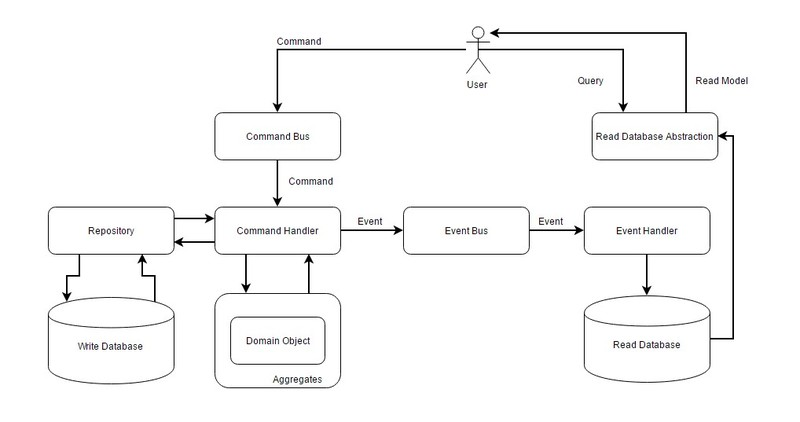
\includegraphics[width=1.0\textwidth]{images/cqrs.jpg}
  \caption{Graficzna reprezentacja wzorca CQRS. Źródło: \cite{EventSourcing1} }
\end{figure}

\section{Java}
,,Java - współbieżny, oparty na klasach, obiektowy język programowania ogólnego zastosowania[4]. Został stworzony przez grupę roboczą pod kierunkiem Jamesa Goslinga z firmy Sun Microsystems. Java jest językiem tworzenia programów źródłowych kompilowanych do kodu bajtowego, czyli postaci wykonywanej przez maszynę wirtualną. Język cechuje się silnym typowaniem. Jego podstawowe koncepcje zostały przejęte z języka Smalltalk (maszyna wirtualna, zarządzanie pamięcią) oraz z języka C++ (duża część składni i słów kluczowych).''\cite{java}

W pracy została użyta Java w wersji 10, która wprowadza pewne usprawnienia widoczne zwłaszcza w implementacji przykładowej aplikacji w wersji opartej na Event Sourcing'u\index{Event Sourcing}, gdzie często używana jest instrukcja "var" dla zmiennych lokalnych.


\begin{figure}[!htb]
  \centering
    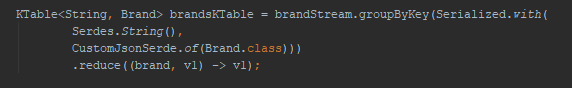
\includegraphics[width=1.0\textwidth]{images/java102.PNG}
  \caption{Standardowa deklaracja zmiennej. Źródło: opracowanie własne}
\end{figure}
\begin{figure}[!htb]
  \centering
    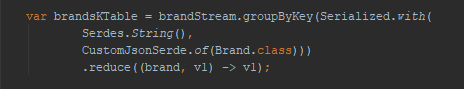
\includegraphics[width=1.0\textwidth]{images/java10.PNG}
  \caption{Deklaracja zmiennej w Javie 10. Źródło: opracowanie włąsne}
\end{figure}

\section{REST}
,,REST – Representational State Transfer – styl architektury oprogramowania opierający się na zbiorze wcześniej określonych reguł opisujących jak definiowane są zasoby, a także umożliwiających dostęp do nich. Został on zaprezentowany przez Roya Fieldinga w 2000 roku.''\cite{restApi}

\section{API}
,,API – Application Programming Interface – zestaw reguł definiujący komunikację pomiędzy programami komputerowymi.

Czyli API są to reguły określające jak użytkownik może uzyskać dostęp do zasobów oraz w jakiej postaci je otrzymuje. Natomiast REST to styl architektury definiujący jak zbudowane będzie to API.''\cite{restApi}

\section{HTTP}
,,HTTP – Hypertext Transfer Protocol – protokół, z którego korzystasz codziennie (lub też jego wersji szyfrowanej – HTTPS) podczas przeglądania stron w sieci. Podczas tworzenia REST API do komunikacji z API wykorzystuje się metody HTTP, których łącznie jest 9. Niemniej jednak do zbudowania podstawowego API pozwalającego na odczyt, zapis, aktualizację i usuwanie danych wystarczą tylko 4 metody – GET, POST, PUT i DELETE.''\cite{restApi}

\section{Spring Framework}

Spring\index{Spring} jest platformą złożoną z wielu projektów, która dedykowana jest do tworzenia aplikacji w języku Java. Jego kluczowym elementem jest kontener wstrzykiwania zależności, jednak przez lata Spring\index{Spring} zyskał wsparcie dla wielu technologii i stanowi dziś jeden z kluczowych elementów całego ekosystemu Javy.\cite{JavaStart-Spring}

\subsection{Moduły Springa użyte w pracy}
Spring sklada się z paru modułów, które odpowiadają za daną funkcjonalność m.in. łączenie z bazą danych i udostępnianie REST API. Aautor pracy wykorzystał następujące moduły Springa\index{Spring}:

\subsubsection{Spring Data}

,,Moduł upraszczający dostęp do baz danych. Główną ideą Spring\index{Spring} Data jest zminimalizowanie ilości powtarzalnego kodu, czyli przykładowo jeśli nasza aplikacja wykorzystuje JPA, potrzebujemy stworzyć repozytorium udostępniające podstawowe metody CRUD\index{CRUD}, to korzystając ze Spring Data całość sprowadza się do stworzenia jednego prostego interfejsu.'' \cite{JavaStart-Spring}


\begin{figure}[h!]
  \centering
    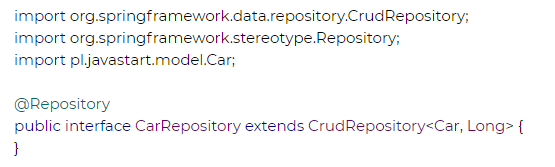
\includegraphics[width=1.0\textwidth]{images/springData.PNG}
  \caption{Repozytorium Spring Data. Źródło: \cite{JavaStart-Spring}}
\end{figure}



\subsubsection{Spring MVC}

 ,,Najpopularniejszy framework MVC (Model View Controller) w Javie. Stanowi alternatywę dla JSF (JavaServer Faces) z Javy EE. Spring\index{Spring} MVC bazuje na technologii serwletów, czyli kluczowej specyfikacji Javy EE i do działania wymaga kontenera serwletów. W najnowszej wersji konfigurację można w całości oprzeć o adnotacje.'' \cite{JavaStart-Spring} Ten moduł wykorzystywany jest w tejże pracy do wystawiania REST API.

\section{Hibernate}

Hibernate to framework do realizacji warstwy dostępu do danych. Zapewnia on translację danych pomiędzy relacyjną bazą danych a światem obiektowym. Opiera się na wykorzystaniu opisu struktury danych za pomocą języka XML lub adnotacji w kodzie, dzięki czemu można rzutować obiekty, stosowane w obiektowych językach programowania, takich jak Java bezpośrednio na istniejące tabele bazy danych. Dodatkowo Hibernate zwiększa wydajność operacji na bazie danych dzięki buforowaniu i minimalizacji liczby przesyłanych zapytań. Jest to projekt open source'owy. \cite{Hibernate}

Hibernate, w połączeniu z modułem Spring\index{Spring} Data, użyty jest do wymiany informacji z bazą danych w aplikacji w wersji monolitycznej\index{aplikacja monolityczna}, przedstawionej w kolejnym rozdziale.

Autor pracy użył Hibernate w połączeniu z adnotacjami w Javie, dzięki czemu nie ma potrzeby definiowania struktury obiektów w plikach o formacie XML.


\begin{figure}[h!]
  \centering
    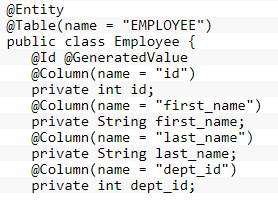
\includegraphics[width=0.5\textwidth]{images/hibernate.PNG}
  \caption{Klasa wraz z adnotacjami Hibernate. Źródło: \cite{Hibernate2}}
\end{figure}



\section{Apache Kafka}

Apache Kafka to open sourceowy broker wiadomości napisany w Javie i Scali.  Kafka w ostatnich latach zyskuje bardzo na popularności ze względu na innowacyjne rozwiązania dotyczące skalowalości i elastyczności rozwiązania. 

,,Cechą charakterystyczną Kafki jest jej niezawodność, wydajność i zdolność do pracy w środowisku rozproszonym. Kiedy zespół LinkedIn tworzył Kafkę, ich główną motywacją było poradzenie sobie z przetwarzaniem w czasie rzeczywistym ogromnej ilości zdarzeń. W konsekwencji powstało narzędzie, które jest idealne do wspomagania przetwarzania dynamicznie zmieniających się źródeł danych o dużej objętości i zmienności, na przykład strumieni big data.

W 2014 roku w LinkedIn komunikacja za pośrednictwem Kafki przebiegała zarówno pomiędzy klastrami, jak i centrami danych. W sumie przesyłano około 200 miliardów komunikatów dzienne, osiągając 7 milionów komunikatów na sekundę, jeśli chodzi o zapis i 35 milionów na sekundę w przypadku odczytu. Z Kafki, poza LinkedIn, korzystają między innymi Netflix, Twitter, Spotify, Cisco, czy Coursera.''\cite{Kafka}

\subsection{Architektura Kafki}

Kafka umożliwia przesyłanie komunikatów pomiędzy aplikacjami w systemach rozproszonych. Nadawca może przesyłać komunikaty do Kafki, a odbiorca pobierać wiadomości ze strumienia publikowanego przez Kafkę.

\subsubsection{Tematy}
Komunikaty pogrupowane są w tzw. tematy (ang. topic). Nadawca przesyła komunikaty z określonego tematu, a odbiorca otrzymuje za pośrednictwem Kafki wszystkie komunikaty z określonego tematu, które mogą pochodzić nawet od wielu nadawców. Każdy wysłany przez dowolnego nadawcę komunikat z danego tematu trafi do każdego odbiorcy, który nasłuchuje tego tematu. Całość odbywa się w środowisku rozproszonym, czyli opratym o mikroserwisy.\cite{Kafka}

\subsubsection{Partycje}
,,Komunikaty z danego tematu dopisywane są do tzw. partycji (ang. partition). Partycja to pewien rejestr, uporządkowana sekwencja komunikatów, która nie zmienia się, oprócz tego, że nowe komunikaty mogą zostać dopisane na koniec tej sekwencji, a stare – na przykład starsze niż dwa dni – są zapominane. Aby pobrać odpowiednią sekwencję komunikatów, odbiorcy muszą jedynie znać swoją pozycję w rejestrze – indeks ostatnio odczytanego komunikatu.

Pojedyncza partycja musi w całości zmieścić się na jednym serwerze, musi być możliwe obsłużenie jej przez jednego brokera. Z innej strony, jeśli masz jedną partycję z jednego tematu, do zapisu i odczytu komunikatów będzie wykorzystywany tylko jeden broker. Większa liczba partycji pozwala na wykorzystanie większej liczby brokerów w celu zrównoleglenia zapisu i odczytu komunikatów, a tym samym na zwiększenie wydajności klastra. Twórcy gwarantują wydajne działanie Kafki nawet dla 10 000 partycji – maksymalnie dla takiej ilości przeprowadzają testy wydajnościowe.''\cite{Kafka}

Partycje Kafki są replikowalne i ich kopie mogą znajdować się na wielu serwerach. Dla każdej partycji istnieje jeden serwer, który jest tzw. liderem (ang. leader) i który obsługuje wszystkie operacje odczytu i zapisu danej partycji. Dla każdej partycji mogą istnieć także serwery (ang. followers), które jedynie replikują dane od lidera.\cite{Kafka} 

\begin{figure}[h!]
  \centering
    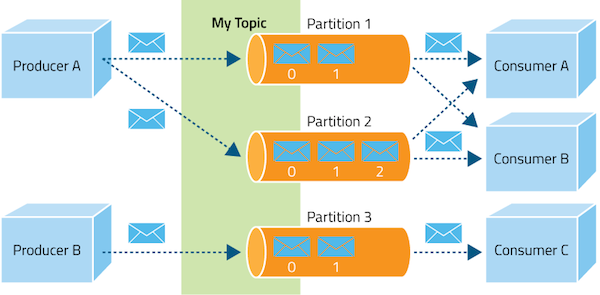
\includegraphics[width=1.0\textwidth]{images/kafka2.png}
  \caption{Relacja między tematem a partycją w Apache Kafka. Źródło: \cite{Kafka2}}
\end{figure}

\subsection{Kafka Core APIs}
\begin{figure}[h!]
  \centering
    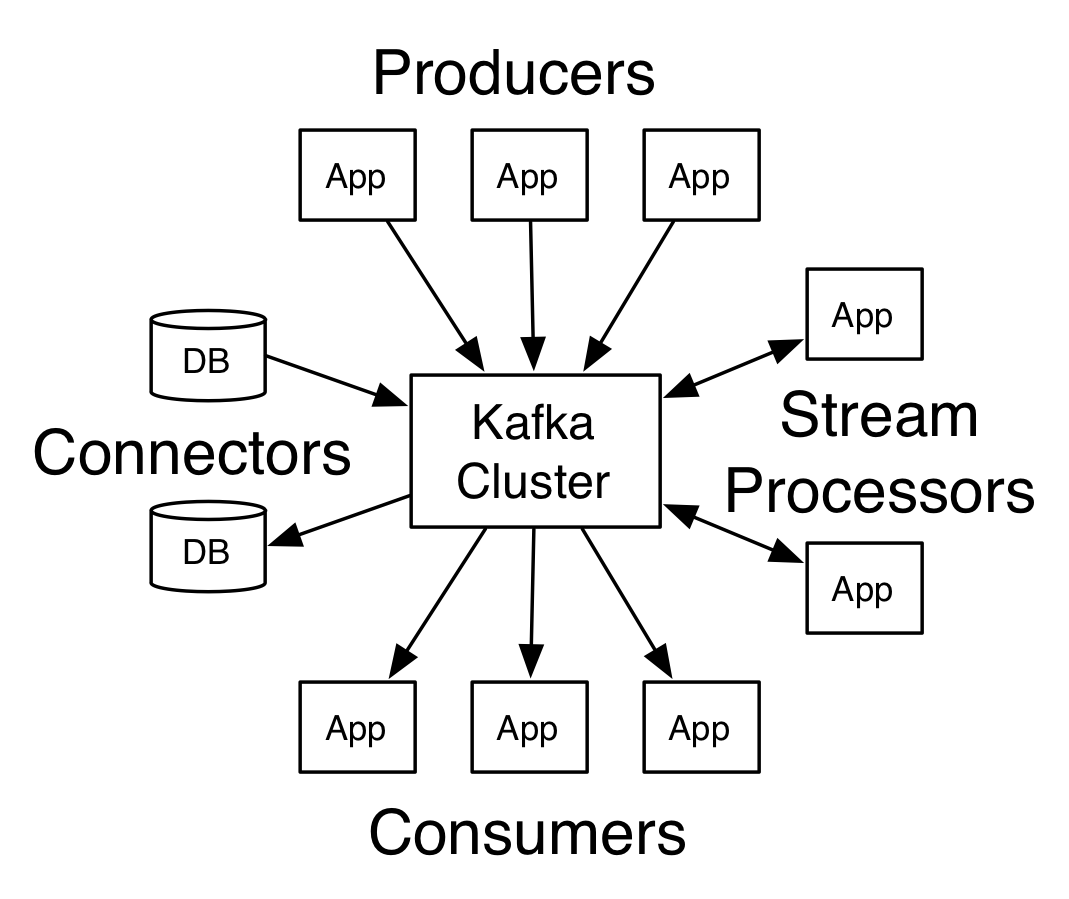
\includegraphics[width=0.5\textwidth]{images/kafka-apis.png}
  \caption{Apache Kafka API. Źródło: \cite{Kafka2}}
\end{figure}

Kafka ma cztery podstawowe API \cite{Streams2}:

\begin{itemize}
    \item Procucer API umożliwia aplikacji publikowanie strumienia rekordów do jednego lub więcej tematów Kafki.
    \item Consumer API pozwala aplikacji subskrybować jeden lub więcej tematów i przetwarzać strumień wygenerowanych rekordów.
    \item Streams API pozwala aplikacji działać jako procesor strumieniowy, pochłaniając strumień wejściowy z jednego lub więcej tematów i generując strumień wyjściowy do jednego lub większej liczby tematów wyjściowych, skutecznie przekształcając strumienie wejściowe w strumienie wyjściowe.
    \item Connector API umożliwia budowanie i uruchamianie producentów lub konsumentów wielokrotnego użytku, łączących tematy Kafki z istniejącymi aplikacjami lub systemami danych. Na przykład łącznik do relacyjnej bazy danych może przechwytywać każdą zmianę w tabeli.
\end{itemize}

W niniejszej pracy zostały wykorzystane Producer API i Streams API, które zostały opisane poniżej.

\subsubsection{Producer API}
Jego główną funkcją jest mapowanie każdej wiadomości na partycję tematu i wysyłanie wydarzenia do lidera tej partycji. Najpierw zostaje obliczona partycja na podstawie klucza, gdzie wydarzenie ma zostać umieszczone. Partycje dostarczane z Kafką gwarantują, że wszystkie wiadomości z tym samym niepustym kluczem zostaną wysłane na tę samą partycję. Jeśli nie podano klucza, partycja jest wybierana w sposób zbalansowany, aby zapewnić równomierną dystrybucję między partycjami tematów.\cite{Producer}

\begin{figure}[h!]
  \centering
    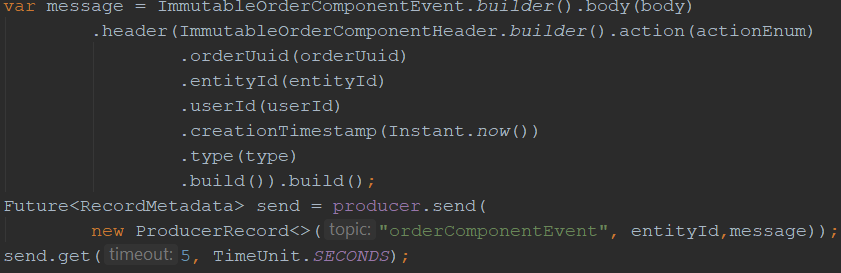
\includegraphics[width=1.0\textwidth]{images/producerexample.PNG}
  \caption{Przykładowe Producer API w Javie. Źródło: opracowanie własne}
\end{figure}
\FloatBarrier

\subsubsection{Streams API}

Kafka Streams jest biblioteką klienta do przetwarzania i analizy danych przechowywanych w Kafce. Opiera się na ważnych koncepcjach przetwarzania strumienia, takich jak odpowiednie rozróżnianie czasu zdarzenia i czasu przetwarzania, obsługa okien i proste, ale wydajne zarządzanie i sprawdzanie w czasie rzeczywistym stanu aplikacji.\cite{Streams}

Kafka posiada wbudowaną możliwość operacji na strumieniach zdarzeń (ang. Streams) i możemy definiować dowolną ilość procesorów (ang. Stream Processors). 


Strumień jest najważniejszą abstrakcją dostarczaną przez Streams API: reprezentuje nieograniczony, stale aktualizowany zbiór danych. Strumień jest uporządkowaną, powtarzalną i odporną na uszkodzenia sekwencją niezmiennych rekordów danych, w której rekord danych jest definiowany jako para klucz-wartość.

Aplikacja do przetwarzania strumienia to dowolny program korzystający z biblioteki Streams API. 
Definiuje swoją logikę obliczeniową przez jedną lub więcej topologii procesora, gdzie topologia jest definicją łączącą procesory strumieniowe.

Procesor strumienia jest węzłem w topologii procesora; reprezentuje on etap przetwarzania w celu transformacji danych w strumieniach przez otrzymywanie jednego rekordu wejściowego w tym samym czasie od jego przyszłych procesorów w topologii, stosując do niego swoją operację, i może następnie wytwarzać jeden lub większą liczbę rekordów wyjściowych w swoich procesorach końcowych.\cite{Streams}

\begin{figure}[h!]
  \centering
    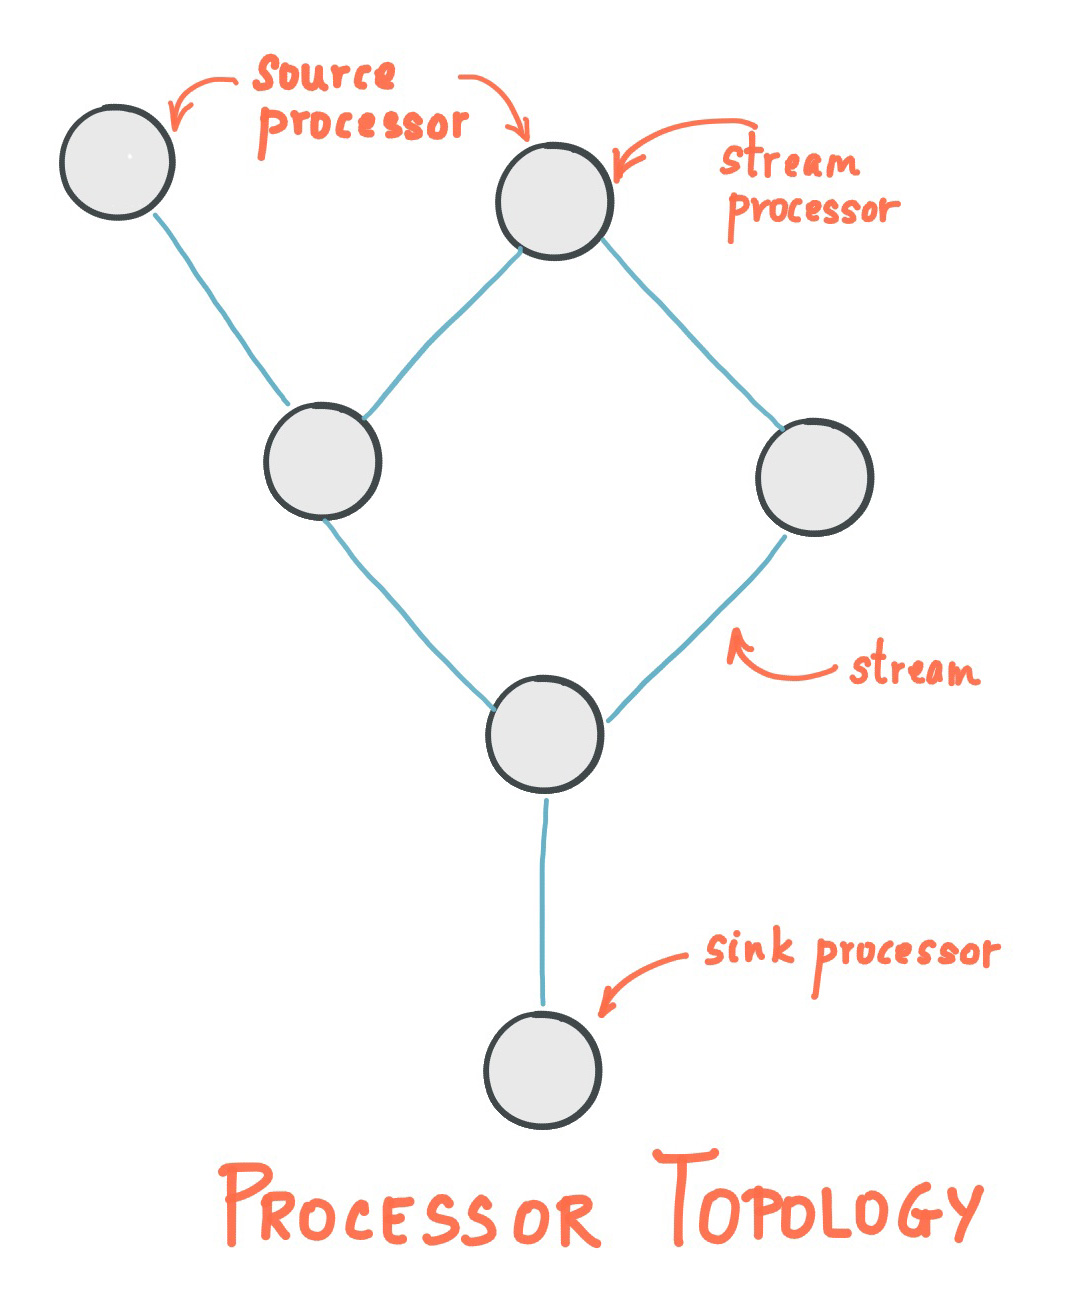
\includegraphics[width=0.5\textwidth]{images/streams.jpg}
  \caption{Topologia procesora w Apache Kafka. Źródło: \cite{Streams}}
\end{figure}
\FloatBarrier

\begin{figure}[h!]
  \centering
    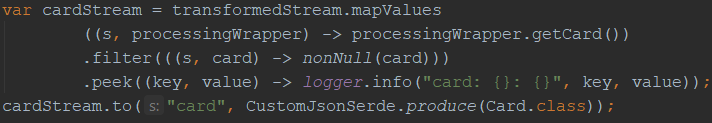
\includegraphics[width=1.0\textwidth]{images/streamexample.PNG}
  \caption{Przykładowe Stream API w Javie. Źródło: opracowanie własne}
\end{figure}
\FloatBarrier


\subsubsection{Dualność strumeni i tabel w Kafce}
Podczas implementowania przypadków użycia strumienia w praktyce zazwyczaj jest potrzeba użycia zarówno strumieni, jak i baz danych. Przykładem, który jest bardzo popularny w praktyce, jest aplikacja e-commerce, która wzbogaca przychodzący strumień transakcji klientów o najnowsze informacje o klientach z tabeli bazy danych. Innymi słowy, strumienie są wszędzie, jak i bazy danych.

Każda technologia przetwarzania strumieniowego musi zatem zapewniać wysokiej klasy obsługę strumieni i tabel. Kafka's Streams API zapewnia taką funkcjonalność poprzez podstawowe abstrakcje obu pojęć. Interesującą obserwacją jest to, że istnieje ścisły związek między strumieniami i tabelami, tak zwana dwoistość strumieniowo-tabelowa. Kafka wykorzystuje tę dwoistość na wiele sposobów: na przykład, aby uczynić aplikacje elastycznymi, aby wspierać przetwarzanie stanowe z tolerancją na błędy lub aby uruchamiać interaktywne zapytania wobec najnowszych wyników przetwarzania aplikacji. Poza swoim wewnętrznym wykorzystaniem API Kafka Streams umożliwia deweloperom wykorzystanie tej dwoistości w swoich własnych aplikacjach. \cite{StreamsConcept}

Dualizm tabeli i strumieni opisuje bliskie relacje między strumieniami i tabelami: \cite{StreamsConcept}
\begin{itemize}
    \item Strumień jako tabela - Strumień można uznać za dziennik zmian danej tabeli, w której każdy rekord danych w strumieniu przechwytuje zmianę stanu tabeli. Strumień można łatwo przekształcić w tabelę, odtwarzając listę zmian od początku do końca, aby zrekonstruować tabelę. Podobnie agregowanie rekordów danych w strumieniu zwróci tabelę. Na przykład możemy obliczyć całkowitą liczbę odsłon użytkownika według strumienia wejściowego zdarzeń odsłon strony, a wynikiem będzie tabela, przy czym kluczem tabeli będzie użytkownik, a wartość będzie odpowiadać liczbie odsłon strony.
    \item Tabela jako strumień: tabelę można uznać za migawkę ostatniej wartości dla każdego klucza w strumieniu (rekordy danych strumienia są parami klucz-wartość). Tabela jest zatem zakamuflowanym strumieniem i można go łatwo przekształcić w "prawdziwy" strumień przez iterowanie po każdym wpisie klucz-wartość w tabeli. 
\end{itemize}

\begin{figure}[h!]
  \centering
    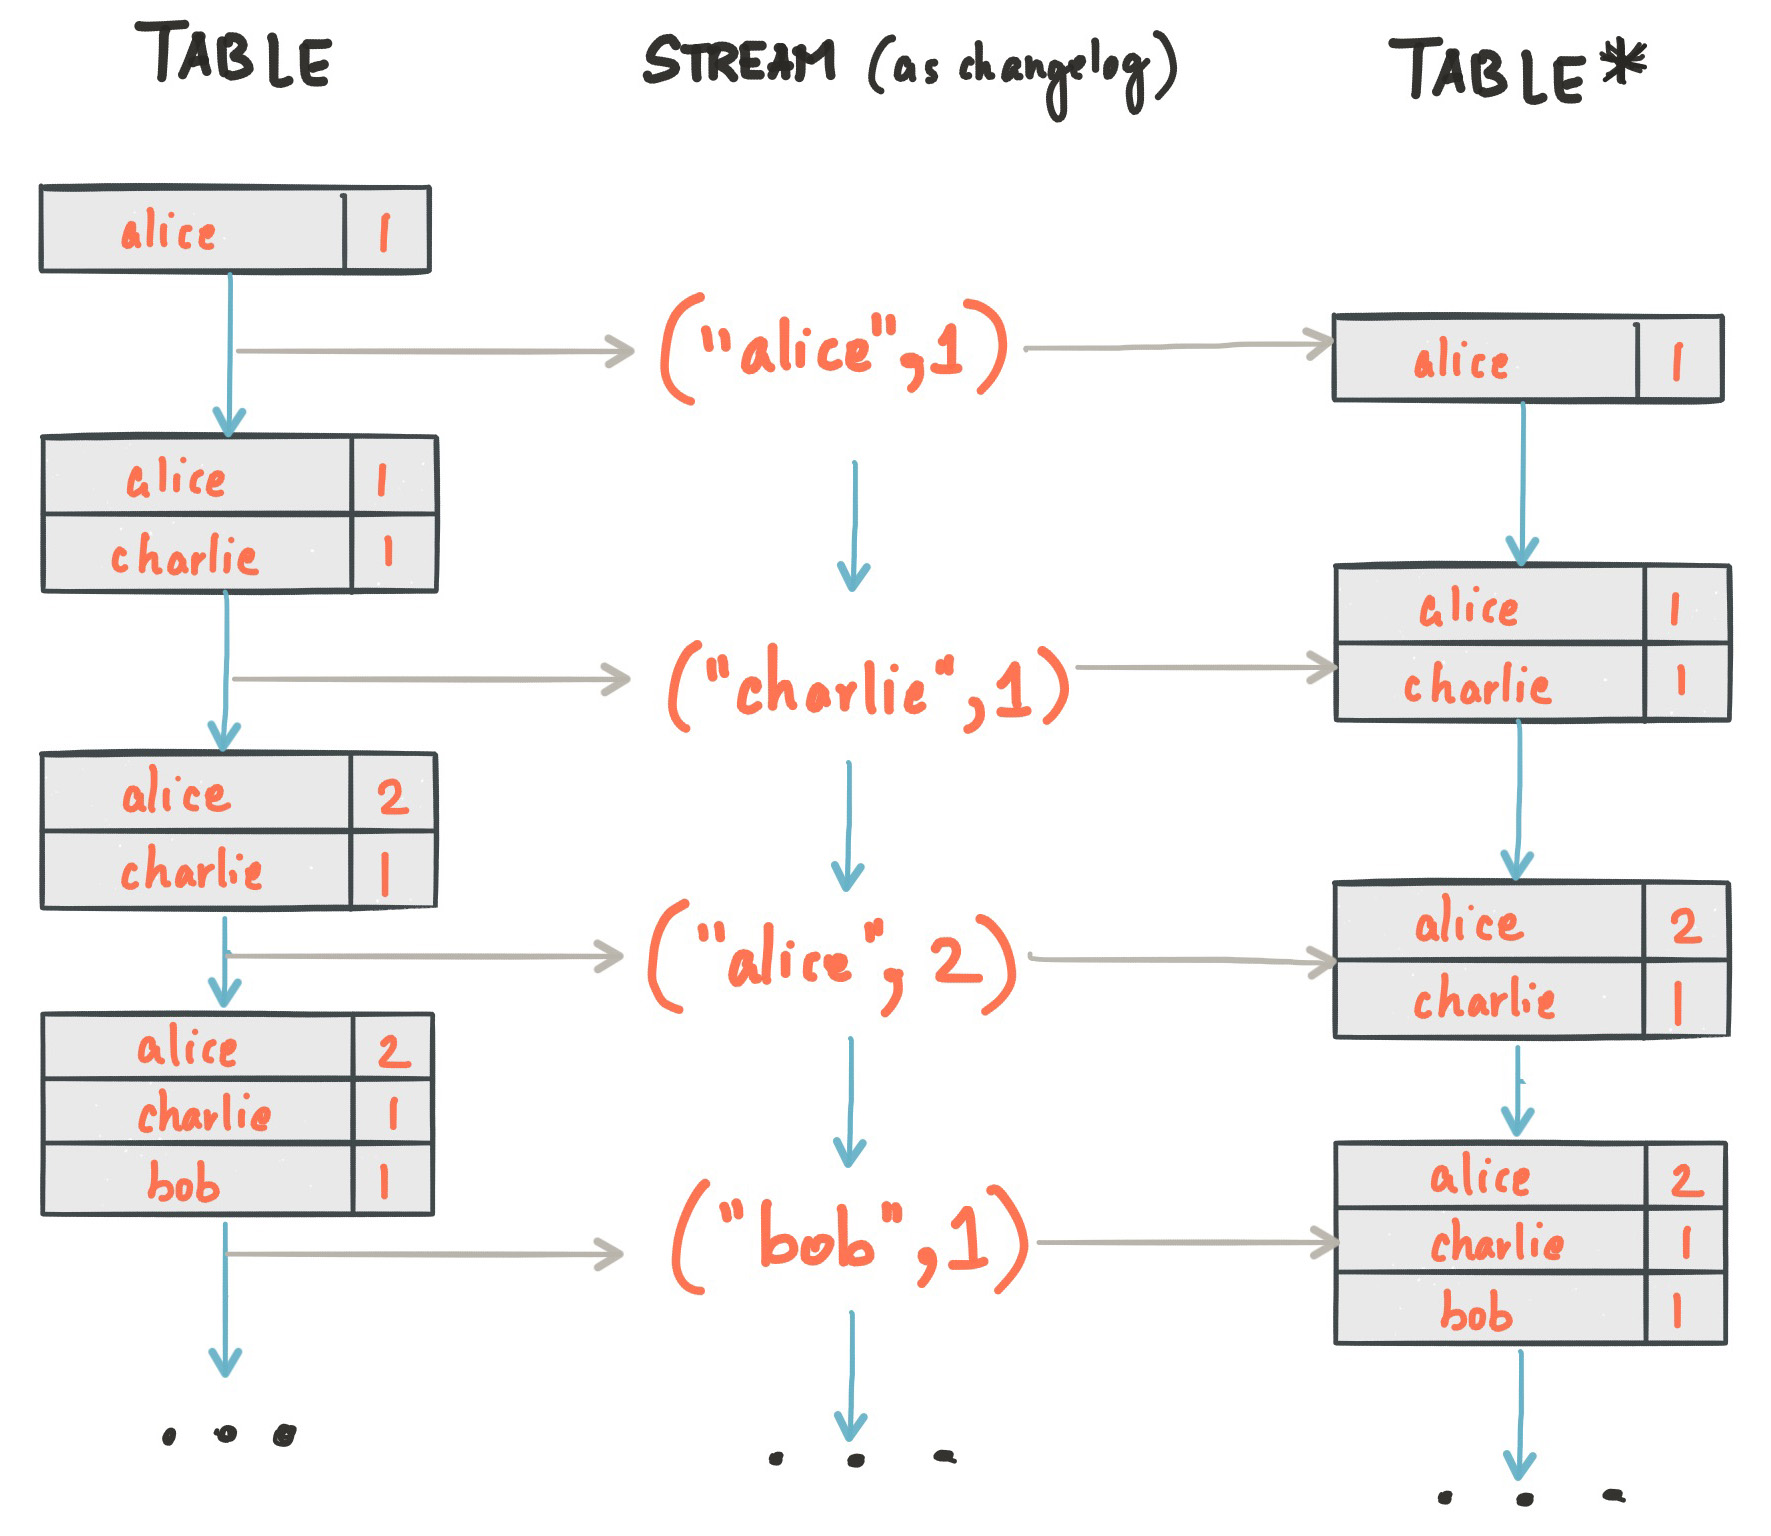
\includegraphics[width=0.7\textwidth]{images/StreamsTableDuality.jpg}
  \caption{Dualizm strumieni i tabel. Źródło: \cite{StreamsConcept} }
\end{figure}
\FloatBarrier

\section{Docker}

Docker to narzędzie zaprojektowane w celu ułatwienia tworzenia, wdrażania i uruchamiania aplikacji przy użyciu kontenerów. Kontenery umożliwiają programistom skompletowanie aplikacji z wszystkimi potrzebnymi częściami, takimi jak biblioteki i inne zależności, i wysłanie jej jako jednej paczki. Dzięki temu, dzięki pojemnikowi, twórca może mieć pewność, że aplikacja będzie działała na dowolnym innym komputerze, niezależnie od dowolnych dostosowanych ustawień, które może mieć maszyna, która może różnić się od maszyny używanej do pisania i testowania kodu.

W pewnym sensie Docker przypomina trochę maszynę wirtualną. Jednak w przeciwieństwie do maszyny wirtualnej, zamiast tworzyć cały wirtualny system operacyjny, Docker pozwala aplikacjom używać tego samego jądra systemu Linux, co system, na którym działają, i wymaga jedynie aplikacji dostarczanych z rzeczami, które nie są jeszcze uruchomione na komputerze hosta. Daje to znaczny wzrost wydajności i zmniejsza rozmiar aplikacji. \cite{Docker}

\subsection{Architektura Docker'owa}
Docker używa architektury klient-serwer. Klient Docker rozmawia z daemonem Docker, który zajmuje się budowaniem, uruchamianiem i dystrybucją kontenerów Docker. Klient i daemon Docker mogą działać w tym samym systemie lub można podłączyć klienta Docker do zdalnego demona Docker. Klient i daemon Docker komunikują się za pomocą REST API lub interfejs sieciowy. \cite{Docker2}

\begin{figure}[h!]
  \centering
    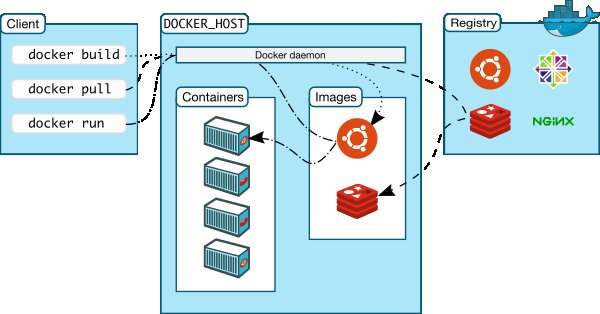
\includegraphics[width=1.0\textwidth]{images/dockerarchitecture.jpg}
  \caption{Architektura Docker'owa. Źródło: \cite{Docker2}}
\end{figure}

\subsubsection{Docker Daemon}
Docker Daemon nasłuchuje żądań interfejsu Docker API i zarządza obiektami Docker, takimi jak obrazy, kontenery, sieci i woluminy. Daemon może również komunikować się z innymi daemonami w celu zarządzania usługami Docker. \cite{Docker2}

\subsubsection{Klient Docker'owy}
Klient Docker'owy to podstawowy sposób interakcji wielu użytkowników Docker z Dockerem. Podczas korzystania z poleceń, takich jak uruchamianie dokera, klient wysyła te polecenia do dockerd, który je wykonuje. Polecenie ,,docker'' używa interfejsu API Docker. Klient Docker'owy może komunikować się z więcej niż jednym deamonem. \cite{Docker2}


\subsubsection{Rejestry Docker'owe}
Rejestr Docker'owy przechowuje obrazy Docker'owe. Docker Hub i Docker Cloud są publicznymi rejestrami, z których każdy może korzystać, a Docker jest domyślnie skonfigurowany do wyszukiwania obrazów w Docker Hub. Możesz nawet uruchomić swój prywatny rejestr. 

Podczas korzystania z poleceń otwierania okna dokowanego lub poleceń dokowania wymagane obrazy są pobierane ze skonfigurowanego rejestru. Po użyciu polecenia ,,push'' obraz zostanie przekazany do skonfigurowanego rejestru.

Sklep Docker pozwala kupować i sprzedawać obrazy Docker lub dystrybuować je za darmo. Na przykład można kupić obraz Docker zawierający aplikację lub usługę od dostawcy oprogramowania i użyć obrazu do wdrożenia aplikacji w środowiskach deweloperskich, testowych i produkcyjnych.

\subsubsection{Obiekty Docker'owe}
Podczas korzystania z Docker tworzysz i używasz obrazów, kontenerów, sieci, woluminów, wtyczek i innych obiektów.

Obraz jest szablonem tylko do odczytu z instrukcjami dotyczącymi tworzenia kontenera Docker'owego. Często obraz jest oparty na innym obrazie, z dodatkową dostosowaną konfiguracją do danych potrzeb.

Można tworzyć własne obrazy lub korzystać tylko z tych stworzonych przez innych i opublikowanych w rejestrze. Aby zbudować własny obraz, należy utworzyć plik Dockerfile z prostą składnią do definiowania kroków potrzebnych do utworzenia obrazu i uruchomienia go. Każda instrukcja w pliku Dockerfile tworzy warstwę na obrazie. Gdy zmienisz plik Dockerfile i odbudujesz obraz, odbudowane zostaną tylko te warstwy, które się zmieniły. Jest to część tego, co sprawia, że obrazy są tak lekkie, małe i szybkie, w porównaniu do innych technologii wirtualizacji.

Kontener to działająca instancja obrazu. Za pomocą interfejsu API lub interfejsu CLI można tworzyć, uruchamiać, zatrzymywać, przenosić i usuwać kontenery. Możesz podłączyć kontener do jednej lub wielu sieci, dołączyć do niego pamięć masową, a nawet utworzyć nowy obraz w oparciu o jego aktualny stan.

Domyślnie kontener jest stosunkowo dobrze izolowany od innych kontenerów i komputera-hosta. Możesz kontrolować sposób odizolowania sieci, kontenera lub innych podstawowych podsystemów od innych kontenerów lub hosta. \cite{Docker2}

\section{Kafka Lenses Box}
Dla łatwości implementacji Event Sourcing'u\index{Event Sourcing}, autor pracy opiera się na gotowym obrazie Docker'owym Apache Kafki, który nazywa się Lenses Box.  

Lenses Box to obraz Docker'owy zawierający pełną instalację Apache Kafki wraz ze wszystkimi jego odpowiednimi komponentami. Wszystko to jest automatycznie skonfigurowane i jedynym wymaganiem jest zainstalowanie Dockera. Zawiera Lenses, brokera Kafki, Kafka Connect, 25+ Kafka Connectors z obsługą SQL, narzędzia CLI. \cite{Lenses}

\section{Swagger}
Aplikacje zaimplementowane na potrzeby tej pracy posiadają jedynie back-end aplikacji bez interfejsu użytkownika napisanego w technolgiach front-endowych. 

Prostym interfejsem, generowanym na podstawie endpoint'ów RESTowych, jest Swagger, który stwarza automatycznie możliwość wysyłania każdego typu zapytania HTTP wraz z zawartością JSON.

\begin{figure}[h!]
  \centering
    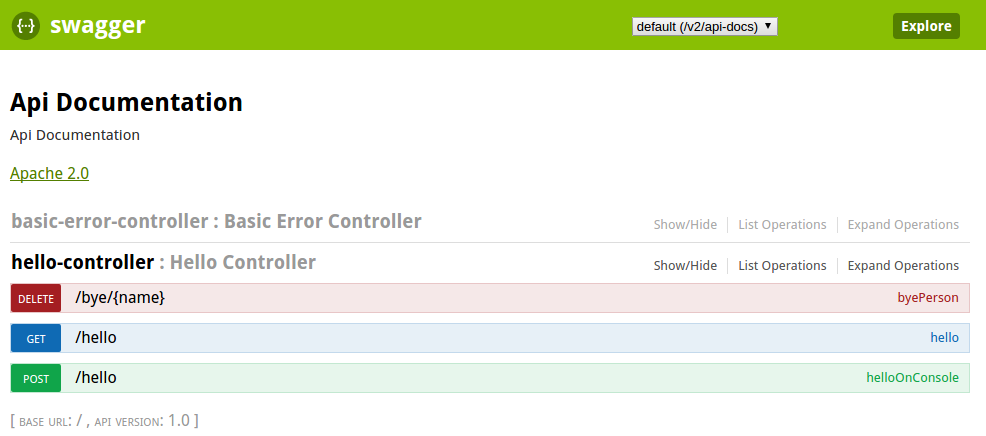
\includegraphics[width=1.0\textwidth]{images/swagger.png}
  \caption{Przykładowy interfejs Swagger'owy. Źródło: \cite{Swagger}}
\end{figure}

\section{Immutables}

Immutables to biblioteka do generowania za pomocą adnotacji niezmiennych obiektów w Javie, czyli takich, których stan nie może zostać zmieniony przez cały okres życia obiektu. 

\begin{figure}[h!]
  \centering
    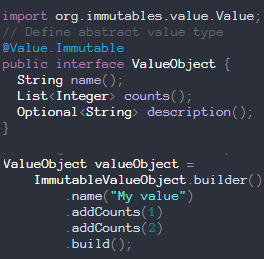
\includegraphics[width=0.6\textwidth]{images/immutables.png}
  \caption{Definicja i tworzenie obiektu niezmiennego. Źródło: \cite{Immutables}}
\end{figure}


\section{Apache Maven}
,,Apache Maven - narzędzie automatyzujące budowę oprogramowania na platformę Java. Poszczególne funkcje Mavena realizowane są poprzez wtyczki, które są automatycznie pobierane przy ich pierwszym wykorzystaniu. Plik określający sposób budowy aplikacji nosi nazwę POM-u (ang. Project Object Model).''\cite{maven} Apache Maven został wykorzystany jako narzędzie do budowania aplikacji w ramach ten pracy. Apache Maven wykorzystuje komendę ,,mvn spring-boot:run'', która buduje i załącza aplikację poprzez wbudowany kontener Tomcat.


